\documentclass[aspectratio=169]{beamer}

\usepackage[utf8]{inputenc}
%\usepackage{emoji}

\usepackage{amsmath}
\usepackage{graphicx}
\usepackage[T1]{fontenc}
\usepackage{libertine}
\usepackage{array}
\usepackage{enumitem}
\usepackage{marvosym}

\setitemize{label=\usebeamerfont*{itemize item}%
  \usebeamercolor[fg]{itemize item}
  \usebeamertemplate{itemize item},
}
\setbeamertemplate{itemize item}[square]
\setbeamertemplate{itemize subitem}[circle]

\usepackage{pgfplots}
\usepackage{tikz}
\usetikzlibrary{automata, arrows, positioning, calc, external, babel, backgrounds, matrix, shapes, shadings}
\usepgfplotslibrary{fillbetween}


%%natbib conf
\usepackage[square,authoryear]{natbib}
\renewcommand{\cite}{\citep}
\renewcommand{\bibfont}{\small}
\bibliographystyle{abbrvnat} 

\newcommand{\R}{\mathbb{R}}
\newcommand{\brackets}[2]{\left\langle#1,#2\right\rangle}
\newcommand{\ind}[1]{\mathbf{1}_{\left\{#1\right\}}}

\newcommand{\graphheight}{7cm}
\newcommand{\graphwidth}{11cm}

\newcommand{\E}[1]{E\left[#1 \right]}
\renewcommand{\phi}{\varphi}

% \definecolor{azulcito}{RGB}{20,70,140}
\definecolor{azulcito}{RGB}{0,90,150}
\definecolor{verdecito}{RGB}{90,150,0}
\definecolor{rojito}{RGB}{150,0,90}
\definecolor{violetita}{RGB}{150,20,150}


\setbeamercolor*{structure}{fg=azulcito,bg=azulcito!20!white}
\setbeamercolor*{alerted text}{fg=azulcito}

  \setbeamercolor{block title}{fg=azulcito,bg=azulcito!20!white}
  \setbeamercolor{block body}{fg=black,bg=azulcito!10!white}
  
\beamertemplatenavigationsymbolsempty

\setbeamercolor*{author in head/foot}{fg=azulcito,bg=azulcito!15!white}
\setbeamercolor*{title in head/foot}{fg=azulcito,bg=azulcito!15!white}
\setbeamercolor*{date in head/foot}{fg=azulcito,bg=azulcito!15!white}

% Pgfplots
\pgfplotsset{width=\graphwidth, height = \graphheight, grid style = {dashed, gray}, every tick label/.append style = {font=\footnotesize}, compat=1.18, legend style={font=\footnotesize, draw=none, fill=none}, every axis/.append style={label style={font=\footnotesize}}}

\tikzset{>=stealth}

\newtheorem{proposition}{Proposition}
%\newtheorem{definition}{Definition}
%\newtheorem{lemma}{Lemma}
%\newtheorem{corollary}{Corollary}

\defbeamertemplate*{footline}{mitema}
{
  \leavevmode%
  \hbox{%
  \begin{beamercolorbox}[wd=.25\paperwidth,ht=2.25ex,dp=1ex,left]{author in head/foot}%
    \usebeamerfont{author in head/foot}\hspace*{2ex}\insertshortauthor
  \end{beamercolorbox}%
  \begin{beamercolorbox}[wd=.5\paperwidth,ht=2.25ex,dp=1ex,center]{title in head/foot}%
    \usebeamerfont{date in head/foot}\insertshortdate{}
  \end{beamercolorbox}%
  \begin{beamercolorbox}[wd=.25\paperwidth,ht=2.25ex,dp=1ex,right]{date in head/foot}%
    \insertframenumber{}/\inserttotalframenumber\hspace*{2em} 
  \end{beamercolorbox}}%
 \vskip0pt%
}


\setbeamercolor{blocky}{fg=azulcito,bg=azulcito!15!white}
\setbeamercolor{blocky2}{fg=black,bg=azulcito!10!white}

\defbeamertemplate*{title page}{customized}[1][]
{
{\flushright
  \begin{beamercolorbox}[wd=\paperwidth,sep=1em,right,rightskip=1.5em]{blocky}%
    \usebeamerfont{title}{\huge \inserttitle}\par \bigskip

    \usebeamerfont{subtitle}{\large \insertsubtitle}\par
  \end{beamercolorbox}%
  \vfill
    \usebeamerfont{author}{\Large \insertauthor}\par \vspace{1em}
      \usebeamerfont{institute}{\large \insertinstitute}\par
  
  
  \vfill
  \usebeamerfont{date}{\insertdate}\par
  %\usebeamercolor[fg]{titlegraphic}\inserttitlegraphic
  }
}

\usefonttheme[onlymath]{serif}

\title{The last, the least and the urgent...}
\subtitle{A story of three policies}

\author[Andres Ferragut, Universidad ORT Uruguay]{Andres Ferragut}
\institute{Joint work with Diego Goldsztajn and Fernando Paganini\\ \smallskip Universidad ORT Uruguay}
\date[INRIA MATHNET Seminar -- Jun 2025]{INRIA MATHNET Seminar -- June 2025}

\AtBeginSection[]
{
\begin{frame}{Outline}
\tableofcontents[currentsection, 
   hideallsubsections, 
   sectionstyle=show/shaded,
]
\end{frame}
}

\newenvironment*{myitem}[1][1.5em]{\begin{itemize}\setlength{\itemsep}{#1}}{\end{itemize}}

\begin{document}

\frame[plain]{\titlepage}

\begin{frame}{Outline}
\tableofcontents
\end{frame}

\section{Introduction}

\begin{frame}{Motivation}{A bit of history...}

	\begin{myitem}
		\item Several queueing systems have service and \alert{timing} requirements.
		\item Examples:
		\begin{itemize}
			\item Computing tasks with real-time constraints.
			\item Item delivery problems in logistics.
			\item Emergency response.
			\item etc. etc. etc.
		\end{itemize}
		\item This has led to a long and rich history of research about \alert{queues with abandonments} \cite{barrer1957queuing,stanford1979reneging,baccellietal1984single}.
	\end{myitem}

\end{frame}

\begin{frame}{Motivation}{Recent developments...}

	One of the most used policies is \alert{Earliest-Deadline-First (EDF)}
	\begin{itemize}
		\item Give priority to tasks with more urgent deadlines.
	\end{itemize}
	\vfill
	\pause
	
	Through fluid limits and diffusion approximations, establish performance:
	\begin{itemize}
		\item \cite{decreusefondmoyal2005fluid} establish EDF fluid limits in the single server case.
		\item \cite{kruketal2011heavy} provides diffusion approximations.
		\item \cite{moyal2013queues} establish some optimality properties of EDF.
		\item \cite{kangramanan2010fluid, kangramanan2012asymptotic} analyze the many-server case.
		\item \cite{ataretal2018law,ataretal2023long} establish asymptotic performance.
	\end{itemize}
	\vfill
	and many others...
\end{frame}

\begin{frame}{Motivation}
	
	\begin{block}{Common assumption}
		\begin{center}
		Customers renege \emph{only} in the queue, and not during service.
		\end{center}
	\end{block}
	\vfill
	\pause

	We call this the \emph{call-center scenario}:

	\begin{itemize}
		\item Akin to waiting for the customer-help line to pick your call while you listen to annoying music.
		
		\item The underlying idea is that when a task reaches service, it will stay until completion.
		
	\end{itemize}
	
	\vfill

	\alert{Key performance metric:} number of satisfied tasks (or reneging probability).

\end{frame}

\begin{frame}{Motivation}{Partial service queues}

	In several queueing systems:

	\begin{itemize}
		\item Tasks may abandon during service.
		\item More importantly, \alert{all service provided may be useful}.
	\end{itemize}

	\vfill

	We call this setting \alert{queues with partial service}.

	\pause

	\vfill

	Some examples:
	\begin{itemize}
		\item Electrical vehicle charging: customers leave the system with a \emph{partial charge}.
		\item LLM inference: longer computation times lead to better answers, but these may be interrupted to deliver a quick response.
		\item File transfers over the Internet, that can be resumed later.
	\end{itemize}

\end{frame}

\begin{frame}{Key points of this talk}
	
	\begin{myitem}
		\item Provide some suitable representation of the state space and dynamics of these partial service queues.
		
		\item Analyze several interesting policies under a suitable fluid model.
		
		\item Compute the main performance metric here: \alert{attained work}.
		
		\item \emph{Last but not least:} show that the simple LCFS policy \alert{exhibits the same performance} than EDF in this setting, without using deadline information. 
	\end{myitem}
\end{frame}

\section{A crash course on measure valued processes}

\begin{frame}{Measure valued stochastic processes}
	
	Consider the simple $M/G/\infty$ queue:
	\begin{itemize}
		\item Tasks arrive as a Poisson process of intensity $\lambda$.
		\item Each task has a service requirement $S\sim g(\sigma)$.
	\end{itemize}
	\vfill
	\begin{center}
		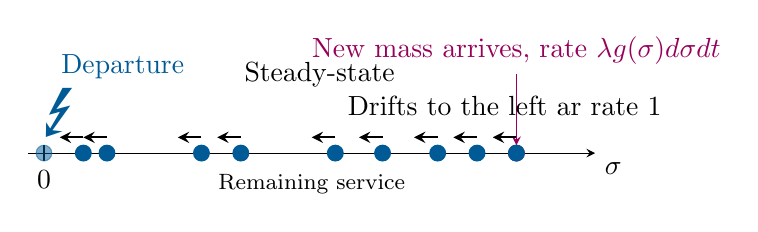
\begin{tikzpicture}    
			\draw [->] (-.2,0) -- node[midway,below,yshift=-1ex]{\footnotesize Remaining service} (7,0);
			\node [below right] at (7,0) {$\sigma$};
			\draw (0,.1) -- (0,-.1) node[below] {$0$};

			\uncover<2>{
				\draw [->,rojito] (6,1) node[above] {New mass arrives, rate $\lambda g(\sigma)d\sigma dt$} -- (6,.1);
				\draw [rojito, fill=rojito] (6,0) circle [radius=0.1];
			}
			\uncover<3>{
				\draw [azulcito, fill=azulcito] (6,0) circle [radius=0.1];
				\draw [thick,->] (6,.2) -- node[midway,above,yshift=1ex] {Drifts to the left ar rate $1$} ++(-.3,0);
			}
			\uncover<4>{
				\draw [azulcito, fill=azulcito, opacity = 0.5, fill opacity=0.5] (0,0) circle [radius=0.1];
				\node[azulcito] at (0.2,0.5) {\Huge\Lightning};
				\node[azulcito] at (1,1.1) {Departure};
			}
			\uncover<5->{
				\foreach \x in {.5,.8,2,2.5,3.7,4.3,5,5.5} {
					\draw [azulcito, fill=azulcito] (\x,0) circle [radius=0.1];
					\draw<5> [thick,->] (\x,.2) --  ++(-.3,0);
				}
				\node at (3.5,1) {Steady-state};
			}

			
		\end{tikzpicture}
	\end{center}
	\vfill
	\uncover<6->{
		\alert{State-descriptor:}
		\begin{equation*}
			\Phi_t = \sum_i \delta_{\sigma_i(t)}
		\end{equation*}
		a Point-process on the positive half-line.
	}
\end{frame}

\begin{frame}{M/G/$\infty$, steady state}
	
	\begin{itemize}
		\item $\Phi_t$ is a measure-valued Markov process.
		\item Its dynamics can be characterized through its generator.
		\item In steady state:
		\begin{equation*}
			\Phi \sim \textrm{Poisson Process with mean measure } \mu(d\sigma) = \lambda \bar{G}(\sigma)d\sigma
		\end{equation*}
		where $\bar{G}$ is the CCDF of $S$.
	\end{itemize}

	\pause
	\vfill
	\alert{Interpretation:}

	\begin{itemize}
	 \item Write $\mu(d\sigma) = \rho \left[\frac{1}{E[S]}(1-G(\sigma))\right]d\sigma$, with $\rho = \lambda E[S]$.
	 \item Then $\left[\frac{1}{E[S]}(1-G(\sigma))\right]d\sigma$ is the \emph{residual service time distribution} associated to $G$.
	 \item In steady-state, the total number of customers $\sim \textrm{Poisson}(\rho)$ and distributed in $\sigma$ as the residual lifetime distribution.
	\end{itemize}

\end{frame}

\begin{frame}{M/G/$\infty$, fluid approximation.}
	
	Suppose that we can replace $\Phi_t$ by a general measure $\mu_t$ with density $f(\sigma;t)$. 
	
	\begin{center}
		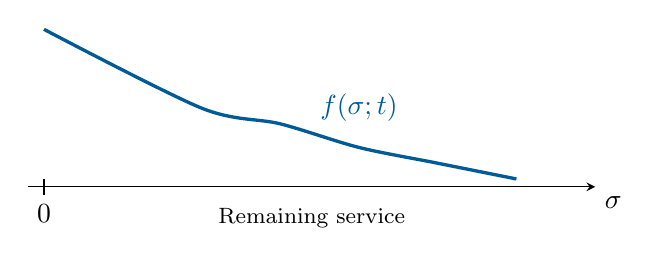
\begin{tikzpicture}    
			\draw [->] (-.2,0) -- node[midway,below,yshift=-1ex]{\footnotesize Remaining service} (7,0);
			\node [below right] at (7,0) {$\sigma$};
			\draw (0,.1) -- (0,-.1) node[below] {$0$};

			\draw [azulcito, very thick] plot [smooth] coordinates {(0,2) (2,1) (3,.8) (4,.5) (5,.3) (6,.1)};
			\node[azulcito] at (4,1) {$f(\sigma;t)$};
		\end{tikzpicture}
	\end{center}
	\begin{itemize}
		\item Mass is transported to the left at rate $1$.
		\item New mass arrives at $\sigma$ with intensity $\lambda g(\sigma)d\sigma dt$.
	\end{itemize}
\vfill
	We can combine this in the following \alert{transport equation}:
	\begin{equation*}
		\frac{\partial f}{\partial t} = \frac{\partial f}{\partial \sigma} + \lambda g(\sigma).
	\end{equation*}

\end{frame}

\begin{frame}{M/G/$\infty$, fluid approximation.}

	Imposing equilibrium and the boundary condition $f(\sigma)\to 0$ as $\sigma\to\infty$ we get:
	\begin{equation*}
		\frac{\partial f}{\partial \sigma} + \lambda g(\sigma) = 0 \Longrightarrow f(\sigma) = \lambda \int_\sigma^{\infty} g(u)\, du = \lambda \bar{G}(\sigma),
	\end{equation*}
	so the fluid approximation recovers the mean measure of $\Phi$.

	\pause\vfill
	\begin{itemize}
		\item This is a deterministic measure, with total mass $\rho$... 
		\item ...distributed in the real line as the residual service distribution.
		\item Serves as an approximation of $\Phi$ in a large scale system ($\lambda\to\infty$).
	\end{itemize}
\end{frame}

\begin{frame}{M/G/$\infty$: take two}{Attained service state descriptor}

	Here is another approach to model the same system \cite{kangramanan2010fluid}:
	\vfill
	\begin{center}
		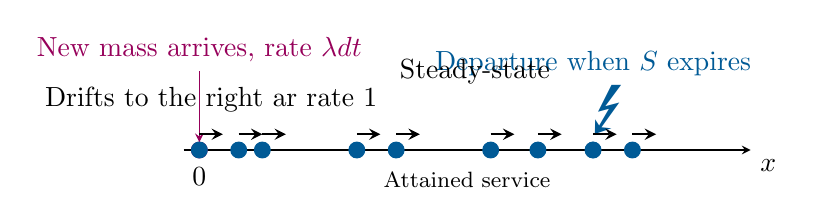
\begin{tikzpicture}    
			\draw [->] (-.2,0) -- node[midway,below,yshift=-1ex]{\footnotesize Attained service} (7,0);
			\node [below right] at (7,0) {$x$};
			\draw (0,.1) -- (0,-.1) node[below] {$0$};

			\uncover<2>{
				\draw [->,rojito] (0,1) node[above] {New mass arrives, rate $\lambda dt$} -- (0,.1);
				\draw [rojito, fill=rojito] (0,0) circle [radius=0.1];
			}
			\uncover<3>{
				\draw [azulcito, fill=azulcito] (0,0) circle [radius=0.1];
				\draw [thick,->] (0,.2) -- node[midway,above,yshift=1ex] {Drifts to the right ar rate $1$} ++(.3,0);
			}
			\uncover<4>{
				\draw [azulcito, fill=azulcito, opacity = 0.5, fill opacity=0.5] (5,0) circle [radius=0.1];
				\node[azulcito] at (5.2,0.5) {\Huge\Lightning};
				\node[azulcito] at (5,1.1) {Departure when $S$ expires};
			}
			\uncover<5->{
				\foreach \x in {.5,.8,2,2.5,3.7,4.3,5,5.5} {
					\draw [azulcito, fill=azulcito] (\x,0) circle [radius=0.1];
					\draw<5> [thick,->] (\x,.2) --  ++(.3,0);
				}
				\node at (3.5,1) {Steady-state};
			}

			
		\end{tikzpicture}
	\end{center}
	\vfill
	\uncover<6->{
		\alert{State-descriptor:}
		\begin{equation*}
			\tilde{\Phi}_t = \sum_i \delta_{x_i(t)}
		\end{equation*}
		a Point-process on the positive half-line, where $x_i(t)$ is the elapsed time in the system
	}

\end{frame}

\begin{frame}{M/G/$\infty$, take two}{Steady-state}
	
	$\tilde\Phi_t$ is a measure-valued Markov process.

	\begin{itemize}
		\item Mass always arrive at $0$ with rate $\lambda dt$.
		\item Transports to the right at rate $1$.
		\item Leaves the system at rate $h(x)$, the \alert{hazard rate function}:
		\begin{equation*}
			h(x) = \lim_{dt\to 0} P(S\in[x,x+dt]\mid S>x) = \frac{g(x)}{\bar{G}(x)} = -\frac{\partial}{\partial x} \log \bar{G}(x).
		\end{equation*}
	\end{itemize}

	\pause
	\vfill
	\alert{Steady-state:}
		\begin{equation*}
			\tilde\Phi \sim \textrm{Poisson Process with mean measure } \nu(dx) = \lambda \bar{G}(x)dx
		\end{equation*}
	
	
	\vfill

	So the reversed representation has the same distribution, because in a random point in time the elapsed service and the remaining service have the same distribution.

\end{frame}


\begin{frame}{M/G/$\infty$: take two}{Fluid approximation.}
	
	Suppose that we can replace $\tilde\Phi_t$ by a general measure $\nu_t$ with density $\tilde f(x;t)$. 
	
	\begin{center}
		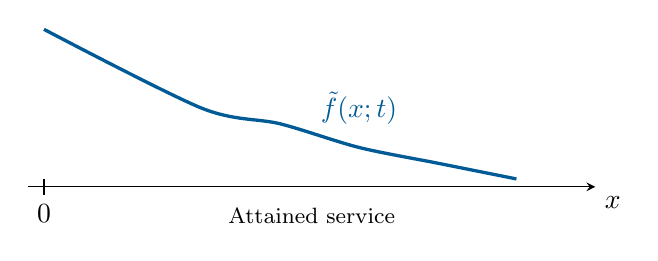
\begin{tikzpicture}    
			\draw [->] (-.2,0) -- node[midway,below,yshift=-1ex]{\footnotesize Attained service} (7,0);
			\node [below right] at (7,0) {$x$};
			\draw (0,.1) -- (0,-.1) node[below] {$0$};

			\draw [azulcito, very thick] plot [smooth] coordinates {(0,2) (2,1) (3,.8) (4,.5) (5,.3) (6,.1)};
			\node[azulcito] at (4,1) {$\tilde f(x;t)$};
		\end{tikzpicture}
	\end{center}
\vfill
\pause
The corresponding transport equation is (informally):
	\begin{equation*}
		\frac{\partial \tilde f}{\partial t} = -\frac{\partial \tilde f}{\partial x} - h(x)\tilde{f} + \lambda \delta_0.
	\end{equation*}
\end{frame}

\begin{frame}{M/G/$\infty$: take two}{Fluid equilibrium.}
	
Imposing equilibrium we get:
	\begin{equation*}
		\frac{\partial \tilde f}{\partial x} = - h(x)\tilde{f} + \lambda \delta_0.
	\end{equation*}

Solving (in a distribution sense) with the boundary condition $\tilde f (\infty) = 0$ we get:
	\begin{equation*}
		\tilde{f}(x) = \lambda e^{-\int_0^x h(u)du}.
	\end{equation*}

But by definition $\int_0^x h(u) du = -\log \bar{G}(x)$, and thus:
	\begin{equation*}
		\tilde{f}(x) = \lambda \bar{G}(x)
	\end{equation*}

So the transport fluid equation recovers again the mean measure of the steady-state.

\end{frame}

\begin{frame}{Lessons learned}

	\begin{myitem}
		\item We can model $M/G$ systems by using two state descriptors:
			\begin{itemize}
				\item The remaining service $\Phi$.
				\item The attained service $\tilde\Phi$.
			\end{itemize}
		\item Both admit reasonable fluid approximations, which correspond to transport equations.
		\item In fact this has been used in the literature to model abandonments (since they operate as $M/G/\infty$ systems in some sense).
	\end{myitem}
	\pause \vfill
	\alert{Question:} can we do more using this machinery of measure-valued processes?
\end{frame}

\section{Partial service queues and Earliest-Deadline-First}

\begin{frame}{Partial service queues}{Setting}

	Consider an $M/G/C$ system where:
	\begin{columns}
		\begin{column}{0.5\textwidth}
			\begin{itemize}
			\item Tasks arrive as a Poisson process of intensity $\lambda$.
			\item<2-> Each task $i$ has two characteristics (marks):
			\begin{itemize}
				\item $S_i$: service time (at rate $1$).
				\item $T_i$: sojourn time or deadline.
			\end{itemize}
			\item<3-> $(S_i,T_i)$ are independent across jobs.
			\item<3-> Follow a common distribution $G(\sigma,\tau)$, possibly correlated.
			\end{itemize} 
		\end{column}
		\begin{column}{0.5\textwidth}

			\begin{tikzpicture}
				\node (arrival) at (0,0) {$\lambda$};
				\node [right of=arrival] (queuel) {};
				\draw[->] (arrival) -- (queuel);
				\draw[thick] (queuel)++(0,.6) --node[midway,above] {Queue} ++(3,0) -- ++(0,-1.2) -- ++(-3,0);

				\foreach \x in {2,2.4,2.8,3.2,3.6} {
					\fill[rojito,thick, fill=rojito!70!white] (\x,.5) rectangle ++(.3,-1);
				}
				\foreach \y in {2,1,0,-1,-2} {
					\draw[azulcito, thick, fill=azulcito!70!white] (5,\y) circle [radius=.4];
				}
				\node[above] at (5,2.5) {$C$ servers};

				\draw<2->[thick,rojito] (2.5,-.75) rectangle ++(1,-1.6);
				\node<2-> at (3,-1.2) {
\includegraphics[width=.5cm]{figuras/battery_mid.png}};
				\node<2-> at (3,-2) {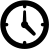
\includegraphics[width=.5cm]{figuras/clock.png}};

				\draw<2->[rojito,thick,->] (2.15,-.5) -- (2.15,-1.6) -- (2.5,-1.6);
			\end{tikzpicture}

		\end{column}
	\end{columns}
\end{frame}

\begin{frame}{Partial service queues}{Definition}

	\begin{block}{Partial service queue}
		Customers depart whenever $S_i$ is attained or the timer $T_i$ expires.
	\end{block}
	\vfill

	\pause
	\begin{myitem}
		\item In particular, they may leave \alert{during service}.

		\item Key performance metrics:
		\begin{myitem}[1em]
			\item \alert{$S_a$}: amount of service \alert{attained}.
			\item Equivalently, \alert{$S_r$}$:=S-S_a$, amount of service \alert{reneged}. 
		\end{myitem}

		\pause

		\item \alert{Problem:} we have to keep track of remaining service and deadlines simultaneously!
	\end{myitem}
\end{frame}


\begin{frame}{System load}

	\begin{myitem}
		
	\item Before proceeding, it is useful to define the \alert{system laod}:

	\begin{equation*}
		\rho:= \lambda E[\min\{S,T\}].
	\end{equation*}

	\pause

	\item \alert{Interpretation:} the mean number of customers on a system with $C=\infty$.

	\item What we expect in a large scale fluid model:
	
	\begin{itemize}
	 \item If $\rho<C$ (underload), all tasks can be served, $S_a = \min\{S,T\}$.
	 \item If $\rho>C$ (overload), demand \emph{curtailing} will occur. How? It depends on the policy...
	\end{itemize}

	\end{myitem}


\end{frame}

\begin{frame}{System evolution}{Remaining service times}

	\begin{columns}
	\begin{column}{0.45\textwidth}
		  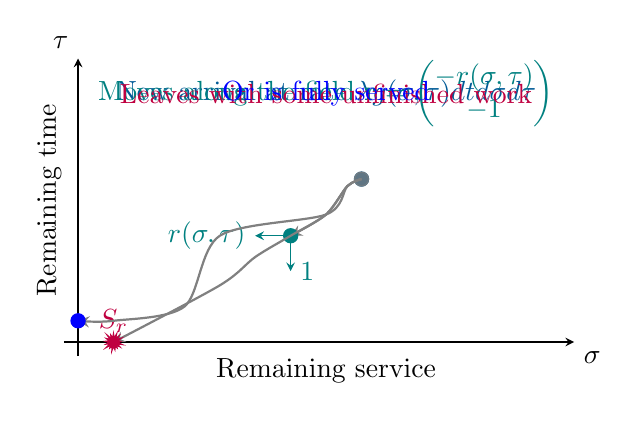
\begin{tikzpicture}[scale=0.9]
    
			\draw [->] (-.2,0) -- (7,0);
			\node [below right] at (7,0) {$\sigma$};
			\draw [->] (0,-.2) -- (0,4);
			\node [above left] at (0,4) {$\tau$};
			
			\node [below] at (3.5,-.1) {Remaining service};
			\node [rotate=90, left, anchor=south] at (-.1,2) {Remaining time};
			
			%	\draw [thick,gray,->] (4,2.3) -- ++(0,-.4);
			\draw<2> [azulcito, fill=azulcito] (4,2.3) circle [radius=0.1];
			\node<2> [azulcito] at (3.5,3.5) {New arrival at rate $\lambda g(\sigma,\tau)dtd\sigma d\tau$};

			\draw<3> [thick,gray,->] plot[smooth] coordinates {(4,2.3) (3.8,2.2) (3.5,1.8) (3,1.5)}; 
			\draw<3> [gray, fill=gray, opacity=0.5] (4,2.3) circle [radius=0.1];
			\draw<3> [teal, fill=teal] (3,1.5) circle [radius=0.1];
			\draw<3> [teal, fill=teal,->] (3,1.5) -- (2.5,1.5) node[left]{$r(\sigma,\tau)$};
			\draw<3> [teal, fill=teal,->] (3,1.5) -- (3,1) node[right]{$1$};
			\node<3> [teal] at (3.5,3.5) {Moves along the field $\mathbf{r} = \begin{pmatrix}
			-r(\sigma,\tau) \\ -1
			\end{pmatrix}$};

			\draw<4> [thick,gray,->] plot[smooth] coordinates {(4,2.3) (3.8,2.2) (3.5,1.8) (3,1.5) (2.5,1.2) (2,.8) (.5,0)}; 
			\draw<4-5> [gray, fill=gray, opacity=0.5] (4,2.3) circle [radius=0.1];
			\node<4>[purple, fill=purple, starburst, inner sep=1.5pt,/pgf/starburst point height=3] at (.5,0) {};
			\node<4>[purple,above] at (.5,0) {$S_r$};
			\node<4> [purple] at (3.5,3.5) {Leaves with some unfinished work};

			\draw<5> [thick,gray,->] plot[smooth] coordinates {(4,2.3) (3.8,2.2) (3.5,1.8) (2,1.5) (1.5,.5) (.5,.3) (0,.3)}; 
			\draw<5> [blue, fill=blue] (0,.3) circle [radius=0.1];
			\node<5> [blue] at (3.5,3.5) {Or is fully served};

		\end{tikzpicture}

	\end{column}
	\begin{column}{0.55\textwidth}
		\begin{itemize}
			\item<1-> Consider the remaining time space.
			\item<3-> \alert{Policy} defines how tasks are served.
			\item<3-> May depend on any combination of $(\sigma,\tau)$.
			\item<5-> State descriptor:
			 \begin{equation*}
				\Phi_t = \sum_i \delta_{\sigma_i(t),\tau_i(t)}
			 \end{equation*}
		\end{itemize}
	\end{column}
	\end{columns}

\end{frame}

\begin{frame}{Example: Earliest-deadline-first}

	\begin{columns}
		\begin{column}{0.45\textwidth}
		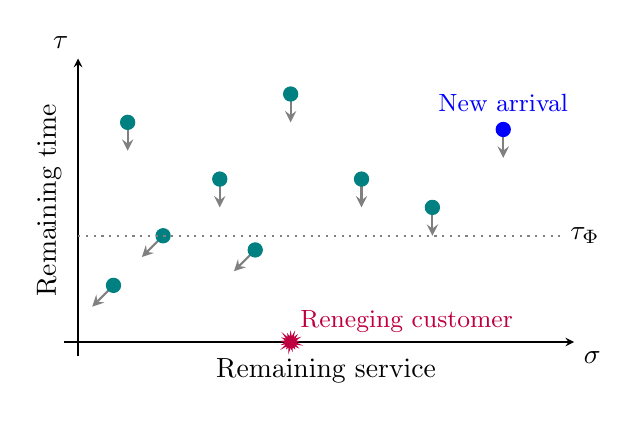
\begin{tikzpicture}[scale=0.9]
				
			\draw [->] (-.2,0) -- (7,0);
			\node [below right] at (7,0) {$\sigma$};
			\draw [->] (0,-.2) -- (0,4);
			\node [above left] at (0,4) {$\tau$};
			
			\node [below] at (3.5,-.1) {Remaining service};
			\node [rotate=90, left, anchor=south] at (-.1,2) {Remaining time};
			
			\draw [thick,gray,->] (.5,.8) -- ++(-.3,-.3);
			\draw [thick,gray,->] (.7,3.1) -- ++(0,-.4);
			\draw [thick,gray,->] (1.2,1.5) -- ++(-.3,-.3);
			\draw [thick,gray,->] (2,2.3) -- ++(0,-.4);
			\draw [thick,gray,->] (2.5,1.3) -- ++(-.3,-.3);
			\draw [thick,gray,->] (3,3.5) -- ++(0,-.4);
			\draw [thick,gray,->] (4,2.3) -- ++(0,-.4);
			\draw [thick,gray,->] (5,1.9) -- ++(0,-.4);
			\draw [thick,gray,->] (6,3) -- ++(0,-.4);

			\draw [teal, fill=teal] (.5,.8) circle [radius=0.1];
			\draw [teal, fill=teal] (.7,3.1) circle [radius=0.1];
			\draw [teal, fill=teal] (1.2,1.5) circle [radius=0.1];
			\draw [teal, fill=teal]  (2,2.3) circle [radius=0.1];
			\draw [teal, fill=teal] (2.5,1.3) circle [radius=0.1];
			\draw [teal, fill=teal] (3,3.5) circle [radius=0.1];
			\draw [teal, fill=teal] (4,2.3) circle [radius=0.1];
			\draw [teal, fill=teal] (5,1.9) circle [radius=0.1];
			\draw [blue, fill=blue] (6,3) circle [radius=0.1] node[above, yshift=3pt] {\small New arrival};

			%reneging departure
			%\draw [purple, fill=purple!20!white] (3,0) circle [radius=0.1] node[above, anchor=south west] {\small Reneging customer};
			\node[purple, fill=purple, starburst, inner sep=1.5pt,/pgf/starburst point height=3] at (3,0) {};
			\node[purple, anchor=south west] at (3,0){ \small Reneging customer};

			\draw [gray, dotted, thick] (0,1.5) -- (6.8,1.5) node[black, right] {$\tau_\Phi$};

		\end{tikzpicture}
	\end{column}
	\begin{column}{0.55\textwidth}
		\begin{itemize}
			\item Serve the $C$ most urgent customers.
			\item Corresponds to taking:
				\begin{equation*}
					r_\Phi(\sigma,\tau) = \mathbf{1}_{\{\tau\leqslant\tau_\Phi\}} 
				\end{equation*}
				with
				\begin{equation*} 
					\tau_\Phi := \sup\{\tau \geqslant 0: \Phi(\mathbb{R}_{+} \times (0, \tau]) < C\}. 	
				\end{equation*} 
		\end{itemize}
	\end{column}
\end{columns}
\end{frame}


\begin{frame}{Fluid model dynamics}
	\begin{itemize}
		\item Replace $\Phi_t$ by a (fluid) measure $\mu_t$.
		\item Now mass drifts along the field:
			\begin{equation*}
				\mathbf{r}_\mu(\sigma,\tau) = \begin{pmatrix}
				-r_\mu(\sigma,\tau) \\
				-1
				\end{pmatrix}
 			\end{equation*}
		\item With $r_\mu$ satisfying:
		\begin{gather*}
			0\leqslant r_{\mu} \leqslant 1 \\
			\iint r_\mu(\sigma,\tau) \mu(d\sigma,d\tau) \leqslant \min\{\mu(\R^2_{++}),C\}.
		\end{gather*} 
	\end{itemize}
\end{frame}

\begin{frame}{Fluid model dynamics}{Weak formulation}

	We will describe these dynamics in terms of the projections 
\begin{equation*}
	\brackets{\phi}{\mu} := \iint \phi(\sigma,\tau) \, \mu(d\sigma,d\tau)
\end{equation*}
of the state measure with  respect to a test function $\phi:\R^2_{++}\to\R$, with continuous derivatives and compact support, i.e. $\phi \in \mathcal{C}^1_c(\R^2_{++})$.  

\vfill

We have:
	\begin{equation*}
	\brackets{\phi}{\mu_{t+dt}} = \iint \phi(\sigma-r_{\mu_t}dt,\tau-dt) \, \mu_{t}(d\sigma,d\tau) + \lambda dt \iint \phi(\sigma,\tau)g(\sigma,\tau)\, d\sigma d\tau + o(dt).
\end{equation*}

\end{frame}

\begin{frame}{Fluid model dynamics}{Weak formulation}

	\begin{align*}
	\frac{\partial}{\partial t}\brackets{\phi}{\mu_{t}} =& \lim_{dt\to 0} \iint \frac{1}{dt} \left[\phi(\sigma-r_{\mu_t}dt,\tau-dt) - \phi(\sigma,\tau)\right] \mu_{t}(d\sigma,d\tau) \\ 
	&+ \lambda \iint \phi(\sigma,\tau)g(\sigma,\tau) d\sigma d\tau\\
=& - \iint \left[r_{\mu_t}(\sigma,\tau) \phi_\sigma (\sigma,\tau) + \phi_\tau(\sigma,\tau)\right]\mu_t(d\sigma,d\tau) + \lambda \iint \phi(\sigma,\tau)g(\sigma,\tau) d\sigma d\tau,
\end{align*}

\end{frame}

\begin{frame}{Fluid model dynamics}{Weak formulation}

	Equivalently:

\begin{align*}
	\brackets{\phi}{\mu_t} = \brackets{\phi}{\mu_0} + \int_0^t &\left[- \iint \left[r_{\mu_s}(\sigma,\tau) \phi_\sigma (\sigma,\tau) + \phi_\tau(\sigma,\tau)\right]\mu_t(d\sigma,d\tau)\right.\\
	& \left. + \lambda \iint \phi(\sigma,\tau)g(\sigma,\tau)\, d\sigma d\tau \right]ds,
\end{align*}
for any $\phi \in \mathcal{C}^1_c(\R^2_{++})$.

\pause
\vfill

Looks daunting, but is not that bad...

\end{frame}

\begin{frame}{Fluid model dynamics}{Transport PDE}

	If $\mu_t$ admits a density $f(\sigma,\tau;t)$ with respect to the Lebesgue measure, it corresponds to:

	\begin{equation*}
		\frac{\partial f}{\partial t} + \nabla \cdot\left[\mathbf{r}_{\mu_t} f\right] = \lambda g
	\end{equation*}
	a transport equation.

	\pause

	\vfill

	\alert{Example: EDF}

	\begin{equation*}
		\frac{\partial f}{\partial t} = \frac{\partial f}{\partial \sigma}\ind{\tau<\tau_{\mu_t}} + \frac{\partial f}{\partial \tau} +\lambda g
	\end{equation*}

\end{frame}

\begin{frame}{EDF Fluid model equilibrium}

	Imposing equilibrium we get:

	\begin{myitem}
		\item $\tau_{\mu^*}=\tau^*$ becomes a constant.
		\item The measure $\mu^*$ must satisfy:
			 \begin{equation*}
				\frac{\partial f}{\partial \sigma}\ind{\tau<\tau^*}  + \frac{\partial f}{\partial \tau} +\lambda g = 0.
			\end{equation*}
		\item Linear PDE that can be easily solved by the method of characteristics.
	\end{myitem}


\end{frame}

\begin{frame}{Solving the EDF transport equation}

	\begin{center}
	
	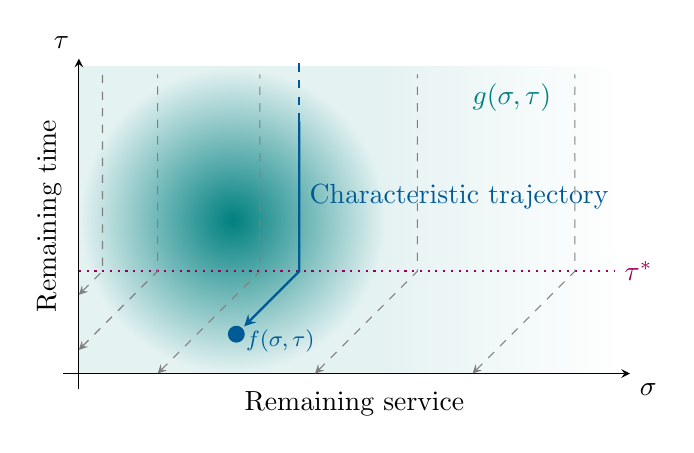
\begin{tikzpicture}
  
	\shade[inner color=teal,outer color=teal!10!white] (0,0) rectangle (3.9,3.9);
	\shade[left color=teal!10!white,right color=white] (3.9,0) rectangle (6.9,3.9);

  \node[teal] at (5.5,3.5) {$g(\sigma,\tau)$};
  \draw [->] (-.2,0) -- (7,0);
  \node [below right] at (7,0) {$\sigma$};
  \draw [->] (0,-.2) -- (0,4);
  \node [above left] at (0,4) {$\tau$};
  
  \node [below] at (3.5,-.1) {Remaining service};
  \node [rotate=90, left, anchor=south] at (-.1,2) {Remaining time};
  
%	\draw [thick,gray,->] (4,2.3) -- ++(0,-.4);
  \draw [rojito, dotted, thick] (0,1.3) -- (6.8,1.3) node[right] {$\tau^*$};
  \draw [azulcito, fill=azulcito] (2,.5) circle [radius=0.1] node[below right, yshift=5pt] {\footnotesize $f(\sigma,\tau)$};

  \draw [azulcito,thick,<-] (2.1,.6) -- (2.8,1.3) -- node[midway, anchor=west] {Characteristic trajectory} (2.8,3.2);
  \draw [azulcito,thick,dashed] (2.8,3.2) -- (2.8,4);

  \draw [gray,dashed,<-] (0,1) -- (.3,1.3) -- (.3,3.8);
  \draw [gray,dashed,<-] (0,.3) -- (1,1.3) -- (1,3.8);
  \draw [gray,dashed,<-] (1,0) -- (2.3,1.3) -- (2.3,3.8);
  \draw [gray,dashed,<-] (3,0) -- (4.3,1.3) -- (4.3,3.8);
  \draw [gray,dashed,<-] (5,0) -- (6.3,1.3) -- (6.3,3.8);

  \end{tikzpicture}
	\end{center}

\end{frame}

\begin{frame}{EDF in overload}{Fluid model equilibrium}

	\begin{theorem}
    Assume that $\rho > C$ and the equation
	\begin{equation*}
		\lambda E[\min\{S,T,\tau^*\}] = C
	\end{equation*}
    has a unique solution $\tau^* > 0$. Consider the measure $\mu^*$ given by the following density:
    \begin{equation*}
		f(\sigma, \tau) = \lambda\left[\int_0^{\left(\tau^* - \tau\right)^+} g(\sigma + u, \tau + u)du + \int_{\left(\tau^* - \tau\right)^+}^\infty g\left(\sigma + \left(\tau^* - \tau\right)^+, \tau + u\right)du\right]. 
	\end{equation*}

	This measure is a fluid equilibrium for the EDF policy, and 
	\begin{equation*}
	\tau^* = \sup \left\{\tau \geq 0:\mu^*(\R_{++} \times (0, \tau]) \leq C\right\}.
	\end{equation*}
	\end{theorem}

\end{frame}

\begin{frame}{EDF performance in equilibrium}
	
	\begin{columns}
		\begin{column}{0.5\textwidth}
		\begin{itemize}
		\item Let us compute the rate at which work is \alert{reneged}.
		
		\item Compute the rate at which mass exits with $S_r < \sigma_0$.
		
		\end{itemize}
		\end{column}
		\begin{column}{0.5\textwidth}
			\begin{tikzpicture}[scale=0.7]
				
			\draw [->] (-.2,0) -- (7,0);
			\node [below right] at (7,0) {$\sigma$};
			\draw [->] (0,-.2) -- (0,4);
			\node [above left] at (0,4) {$\tau$};
			
%			\node [below] at (3.5,-.1) {Remaining service};
%			\node [rotate=90, left, anchor=south] at (-.1,2) { Remaining time};

			\draw [gray, dotted, thick] (0,1.5) -- (6.8,1.5) node[black, right] {$\tau_\Phi$};

			\draw[very thick,rojito] (0,1.5) -- (0,0) -- (2,0);
			\draw[very thick,rojito] (2,.2) -- (2,-.2) node[below]{$\sigma_0$};

			\draw[thick,gray] (2,0) -- (3.5,1.5) -- (3.5,4);

			\draw[thick,gray,->] (1.75,3) -- ++(0,-.9);
			\draw[thick,gray,->] (1.5,1) -- ++(-.6,-.6);

			\end{tikzpicture}
		\end{column}
	\end{columns}

	\begin{proposition}
    \begin{equation*}
        \int_0^{\tau^*} f(0, \tau)d\tau + \int_0^{\sigma_0} f(\sigma, 0)d\sigma = \lambda P\left(S - \min\left\{S, T, \tau^*\right\} < \sigma_0\right).
    \end{equation*}

	\smallskip
	i.e. $S_a = S-S_r = \min\{S,T,\tau^*\}$.
	\end{proposition}
\end{frame}


\section{Deadline-oblivious policies}

\begin{frame}{What if we do not know the deadlines?}

	\begin{myitem}
	\item Deadlines are often hard to estimate in practice.
	\item Moreover, tasks may under-report their deadline to get priority!
	\item What about \alert{deadline-oblivious} policies?
	\begin{itemize}
		\item Can we model them?
		\item What is their performance?
	\end{itemize}
	\end{myitem}
	
	\pause
	\vfill
	\alert{Problem:} we need a new state-space...
\end{frame}


\begin{frame}{Attained service state descriptor}

	\begin{columns}
	\begin{column}{0.45\textwidth}
		  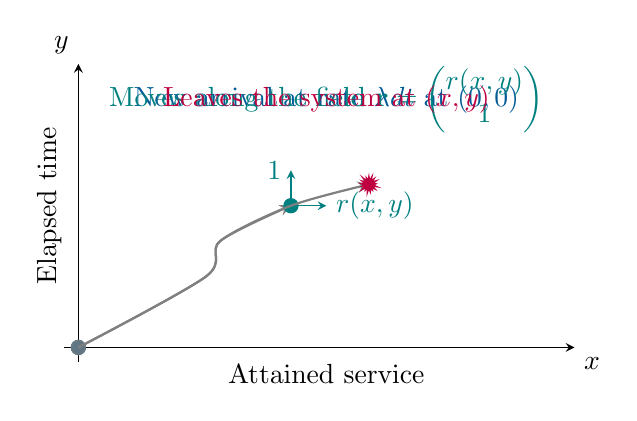
\begin{tikzpicture}[scale=0.9]
		
			\draw [->] (-.2,0) -- (7,0);
			\node [below right] at (7,0) {$x$};
			\draw [->] (0,-.2) -- (0,4);
			\node [above left] at (0,4) {$y$};
			
			\node [below] at (3.5,-.1) {Attained service};
			\node [rotate=90, left, anchor=south] at (-.1,2) {Elapsed time};

			\draw<2> [azulcito, fill=azulcito] (0,0) circle [radius=0.1];
			\node<2> [azulcito] at (3.5,3.5) {New arrival at rate $\lambda dt$ at $(0,0)$};

			\draw<3> [thick,gray,->] plot[smooth] coordinates {(0,0) (1.8,1) (2,1.5) (3,2)}; 
			\draw<3> [gray, fill=gray, opacity=0.5] (0,0) circle [radius=0.1];
			\draw<3> [teal, fill=teal] (3,2) circle [radius=0.1];
			\draw<3> [teal, fill=teal,->] (3,2) -- (3.5,2) node[right]{$r(x,y)$};
			\draw<3> [teal, fill=teal,->] (3,2) -- (3,2.5) node[left]{$1$};
			\node<3> [teal] at (3.5,3.5) {Moves along the field $\mathbf{r} = \begin{pmatrix}
			r(x,y) \\ 1
			\end{pmatrix}$};

			\draw<4-> [thick,gray,->] plot[smooth] coordinates {(0,0) (1.8,1) (2,1.5) (3,2) (4.1,2.3)}; 
			\draw<4-> [gray, fill=gray, opacity=0.5] (0,0) circle [radius=0.1];
			\node<4-> [purple, fill=purple, starburst, inner sep=1.5pt,/pgf/starburst point height=3] at (4.1,2.3) {};
			\node<4-> [purple] at (3.5,3.5) {Leaves the system at $(x,y)$};
			\end{tikzpicture}

	\end{column}
	\begin{column}{0.55\textwidth}
		\begin{itemize}
			\item<1-> Consider the elapsed time space.
			\item<3-> \alert{Policy} again defines how tasks are served.
			\item<3-> May depend on any combination of $(x,y)$.
			\item<5-> State descriptor:
			 \begin{equation*}
				\tilde\Phi_t = \sum_i \delta_{x_i(t),y_i(t)}
			 \end{equation*}
		\end{itemize}
	\end{column}
	\end{columns}

\end{frame}


\begin{frame}{Example: Least-Attained-Service policy}

	\begin{columns}
		\begin{column}{0.45\textwidth}
		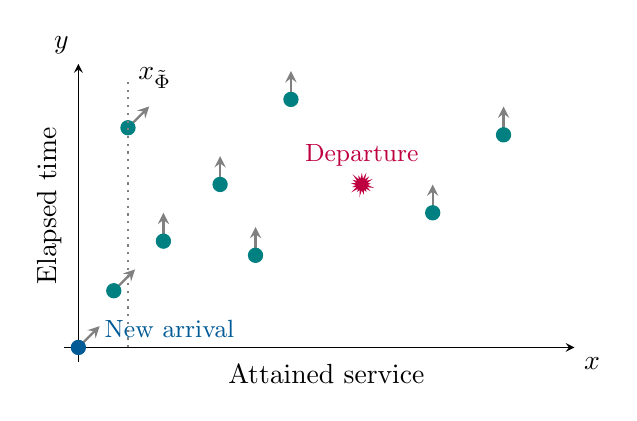
\begin{tikzpicture}[scale=0.9]
			\draw [->] (-.2,0) -- (7,0);
			\node [below right] at (7,0) {$x$};
			\draw [->] (0,-.2) -- (0,4);
			\node [above left] at (0,4) {$y$};
			
			\node [below] at (3.5,-.1) {Attained service};
			\node [rotate=90, left, anchor=south] at (-.1,2) {Elapsed time};
			
			\draw [thick,gray,->] (.5,.8) -- ++(.3,.3);
			\draw [thick,gray,->] (.7,3.1) -- ++(.3,.3);
			\draw [thick,gray,->] (1.2,1.5) -- ++(0,.4);
			\draw [thick,gray,->] (2,2.3) -- ++(0,.4);
			\draw [thick,gray,->] (2.5,1.3) -- ++(0,.4);
			\draw [thick,gray,->] (3,3.5) -- ++(0,.4);
			%\draw [thick,gray,->] (4,2.3) -- ++(.2,.4);
			\draw [thick,gray,->] (5,1.9) -- ++(0,.4);
			\draw [thick,gray,->] (6,3) -- ++(0,.4);

			\draw [teal, fill=teal] (.5,.8) circle [radius=0.1];
			\draw [teal, fill=teal] (.7,3.1) circle [radius=0.1];
			\draw [teal, fill=teal] (1.2,1.5) circle [radius=0.1];
			\draw [teal, fill=teal]  (2,2.3) circle [radius=0.1];
			\draw [teal, fill=teal] (2.5,1.3) circle [radius=0.1];
			\draw [teal, fill=teal] (3,3.5) circle [radius=0.1];
			%\draw [teal!50!white, fill=teal!50!white] (4,2.3) starburst  node[teal,above] {\footnotesize Departure};
			%\node[teal!50!white, fill=teal, starburst, inner sep=1.5pt,/pgf/starburst point height=3] at (4,2.3) {}; 
			%\node[teal,above, yshift=3pt] at (4,2.3) {\footnotesize Departure};
			
			\node[purple, fill=purple, starburst, inner sep=1.5pt,/pgf/starburst point height=3] at (4,2.3) {};
			\node[purple, above, yshift=3pt] at (4,2.3){ \small Departure};
			
			\draw [teal, fill=teal] (5,1.9) circle [radius=0.1];
			\draw [teal, fill=teal] (6,3) circle [radius=0.1];
			
			%new arrival

			\draw [thick,gray,->] (0,0) -- ++(.3,.3);
			\draw [azulcito, fill=azulcito] (0,0) circle [radius=0.1] node[anchor=south west, xshift=6pt] {\small New arrival};
			
			\draw [gray, dotted, thick] (.7,0) -- (.7,3.8) node[black, right] {$x_{\tilde{\Phi}}$};
	\end{tikzpicture}

	\end{column}
	\begin{column}{0.55\textwidth}
		\begin{itemize}
			\item Serve the $C$ least-served tasks.
			\item Corresponds to taking:
				\begin{equation*}
					r_{\tilde\Phi}(x,y) = \mathbf{1}_{\{x\leqslant x_{\tilde\Phi}\}} 
				\end{equation*}
				with
				\begin{equation*} 
					x_{\tilde\Phi} := \sup\{x: \tilde\Phi([0, x] \times \R_+) \leqslant C\}. 	
				\end{equation*} 
		\end{itemize}
	\end{column}
\end{columns}

\end{frame}


\begin{frame}{Example: Last-Come-First-Served policy}
  
	\begin{columns}
		\begin{column}{0.45\textwidth}
			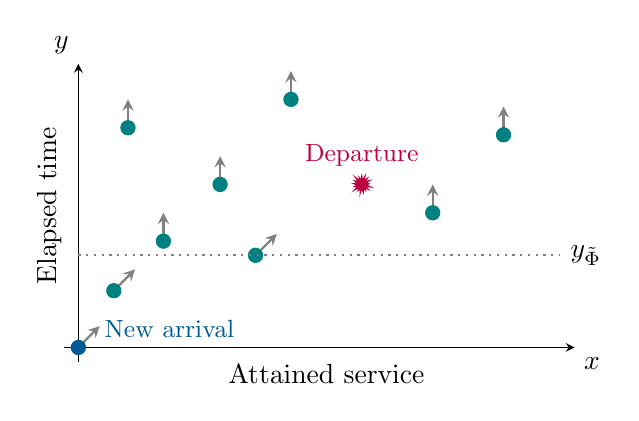
\begin{tikzpicture}[scale=0.9]
					
				\draw [->] (-.2,0) -- (7,0);
				\node [below right] at (7,0) {$x$};
				\draw [->] (0,-.2) -- (0,4);
				\node [above left] at (0,4) {$y$};
				
				\node [below] at (3.5,-.1) {Attained service};
				\node [rotate=90, left, anchor=south] at (-.1,2) {Elapsed time};
				
				\draw [thick,gray,->] (.5,.8) -- ++(.3,.3);
				\draw [thick,gray,->] (.7,3.1) -- ++(0,.4);
				\draw [thick,gray,->] (1.2,1.5) -- ++(0,.4);
				\draw [thick,gray,->] (2,2.3) -- ++(0,.4);
				\draw [thick,gray,->] (2.5,1.3) -- ++(.3,.3);
				\draw [thick,gray,->] (3,3.5) -- ++(0,.4);
				%\draw [thick,gray,->] (4,2.3) -- ++(.2,.4);
				\draw [thick,gray,->] (5,1.9) -- ++(0,.4);
				\draw [thick,gray,->] (6,3) -- ++(0,.4);

				\draw [teal, fill=teal] (.5,.8) circle [radius=0.1];
				\draw [teal, fill=teal] (.7,3.1) circle [radius=0.1];
				\draw [teal, fill=teal] (1.2,1.5) circle [radius=0.1];
				\draw [teal, fill=teal]  (2,2.3) circle [radius=0.1];
				\draw [teal, fill=teal] (2.5,1.3) circle [radius=0.1];
				\draw [teal, fill=teal] (3,3.5) circle [radius=0.1];
				%\draw [teal!50!white, fill=teal!50!white] (4,2.3) starburst  node[teal,above] {\footnotesize Departure};
				%\node[teal!50!white, fill=teal, starburst, inner sep=1.5pt,/pgf/starburst point height=3] at (4,2.3) {}; 
				%\node[teal,above, yshift=3pt] at (4,2.3) {\footnotesize Departure};
				\draw [teal, fill=teal] (5,1.9) circle [radius=0.1];
				\draw [teal, fill=teal] (6,3) circle [radius=0.1];
						
				\node[purple, fill=purple, starburst, inner sep=1.5pt,/pgf/starburst point height=3] at (4,2.3) {};
				\node[purple, above, yshift=3pt] at (4,2.3){ \small Departure};
				
				%new arrival

				\draw [thick,gray,->] (0,0) -- ++(.3,.3);
				\draw [azulcito, fill=azulcito] (0,0) circle [radius=0.1] node[anchor=south west, xshift=6pt] {\small New arrival};
				
				\draw [gray, dotted, thick] (0,1.3) -- (6.8,1.3) node[black, right] {$y_{\tilde{\Phi}}$};
				\end{tikzpicture}
		\end{column}
	\begin{column}{0.55\textwidth}
		\begin{itemize}
			\item Serve the $C$ more recent tasks.
			\item Corresponds to taking:
				\begin{equation*}
					r_{\tilde\Phi}(x,y) = \mathbf{1}_{\{y\leqslant y_{\tilde\Phi}\}} 
				\end{equation*}
				with
				\begin{equation*} 
					y_{\tilde\Phi} := \sup\{y: \tilde\Phi(\R_+\times [0, y]) \leqslant C\}
				\end{equation*} 
		\end{itemize}
	\end{column}
\end{columns}

\end{frame}

\begin{frame}{The hazard rate field}

	We have a new problem: what is the rate at which users \alert{leave} the system?

	\pause

	\vfill

	Let $\bar{G}(x,y) = P(S>x,T>y)$ and define:

	\begin{definition}[Hazard rate field]
		\begin{equation*}
			\mathbf{h}(x,y) = -\nabla \log \bar{G}(x,y)	\quad \text{i.e.}
		\end{equation*}
		\begin{itemize}
			\item $h^x (x,y) = P(S\in[x,x+dx],T>S \mid S>x,T>y)$
			\item $h^x (x,y) = P(T\in[y,y+dy],S>T \mid S>x,T>y)$
		\end{itemize}
	\end{definition}

	\vfill

	Interpretation: $\mathbf{h}$ stores the rate at which $\min\{S,T\}$ is attained due to $S$ or $T$ expiring.
\end{frame}

\begin{frame}{Fluid model dynamics}

	\begin{itemize}
		\item Replace $\tilde{\Phi}_t$ by a (fluid) measure $\nu_t$.
		\item Now mass arrives at $(0,0)$ at rate $\lambda$.
		\item Drifts along the field:
		 \begin{equation*}
			\mathbf{r}_\nu(x,y) = \begin{pmatrix}
				r_\nu (x,y) \\ 1
			\end{pmatrix}
		 \end{equation*}
		 \item With $r_\nu$ satisfying:
		 \begin{gather*}
			0\leqslant r_\nu \leqslant 1 \\
			\iint r_\nu(x,y) \nu(dx,dy) \leqslant \min\{\nu(\R^2_+),C\}.
		 \end{gather*}
	\end{itemize}
\end{frame}

\begin{frame}{Departure rate}

	Now we have to compute the departure rate $\eta_nu(x,y)$:
	\begin{equation*}
		\eta_\nu(x,y) := \lim_{dt\to 0} \frac{1}{dt} P\left(\left\{S\in\left(x,x+r_{\tilde\Phi}dt\right)\right\}\cup \left\{T\in\left(y,y+dt\right)\right\}\mid S>x,T>y\right)
	\end{equation*}

	By the chain rule and some computations:
	\begin{gather*}
		\eta_{\nu}(x,y) =\frac{1}{\bar{G}(x,y)}\left[-\frac{\partial}{\partial x} \bar{G}(x,y) r_{\tilde\Phi}(x,y) - \frac{\partial}{\partial y} \bar{G}(x,y)\right]
	\end{gather*}
	\pause
	Therefore:
	\begin{equation*}
	\eta_{\nu}(x,y) = h^x(x,y)r_{\nu}(x,y)+h^y(x,y) = \mathbf{r}_{\nu}(x,y) \cdot \mathbf{h}(x,y).
	\end{equation*}

\end{frame}

\begin{frame}{Attained service transport equation}

	\begin{myitem}
		\item We now have all ingredients to formulate the dynamics of the system.
		\item The transport equation in the elapsed service space is (informally):
		\begin{equation*}
			\frac{\partial \bar f}{\partial t} + \nabla \cdot\left[\mathbf{r}_{\nu_t} \bar{f}\right] + [\mathbf{r}_{\nu_t}\cdot \mathbf{h}]\bar{f}= \lambda \delta_{(0,0)}.
		\end{equation*}
		where $\tilde{f}$ is the density of $\nu_t$.
		\pause
		\item The above equation must be treated in weak form:
		 \begin{itemize}
			\item To account for the impulse mass at $(0,0)$ driving the system.
			\item To allow solutions without a density as we shall see.
		 \end{itemize}
	\end{myitem}


\end{frame}


\begin{frame}{Last come first served}{Fluid equilibrium}

	Recall that LCFS can be modeled by:
	\begin{equation*}
		r_{\nu}(x, y) = \ind{y < y_\nu}
	\end{equation*}
	with
	\begin{equation*}
	y^* = \sup \left\{y \geq 0: \nu^*(\R_+ \times [0, y]) \leqslant C\right\}.
	\end{equation*}

	\pause
	Imposing equilibrium, $\nu^*$, $y^*$ fixed, we have to solve: 
	\begin{equation*}
		\nabla \cdot\left[\mathbf{r}_{\nu^*} \bar{f}\right] + [\mathbf{r}_{\nu^*}\cdot \mathbf{h}]\bar{f}= \lambda \delta_{(0,0)}.
	\end{equation*}

\end{frame}


\begin{frame}{Solving the transport equation}{Last come first served case}

	\begin{center}
	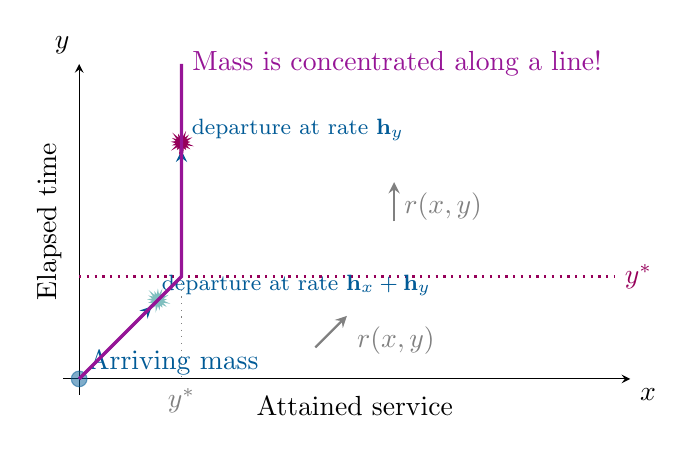
\begin{tikzpicture}
  
		\draw [->] (-.2,0) -- (7,0);
		\node [below right] at (7,0) {$x$};
		\draw [->] (0,-.2) -- (0,4);
		\node [above left] at (0,4) {$y$};
		
		\node [below] at (3.5,-.1) {Attained service};
		\node [rotate=90, left, anchor=south] at (-.1,2) {Elapsed time};

		\draw [gray,thick,->] (3,.4) -- (3.4,.8) node[below right] {$r(x,y)$};
		\draw [gray,thick, ->] (4,2) -- (4,2.5) node[below right] {$r(x,y)$};

		\draw [rojito, dotted, thick] (0,1.3) -- (6.8,1.3) node[right] {$y^*$};
		\draw [azulcito, fill=azulcito, opacity=0.5] (0,0) circle [radius=0.1]; 
		\node<1> [azulcito, anchor=west] at (0,.2) {Arriving mass};
		\draw<2> [azulcito,thick,->] (0,0) -- (.92,.92) node[above right] {\footnotesize departure at rate $\mathbf{h}_x+\mathbf{h}_y$};
		\node<2>[teal!50!white, fill=teal!50!white, starburst, inner sep=1.5pt,/pgf/starburst point height=3] at (1,1) {}; 
		\draw<3> [azulcito,thick,->] (0,0) -- (1.3,1.3) -- (1.3,2.9) node[above right] {\footnotesize departure at rate $\mathbf{h}_y$};
		\node<3>[rojito!50!white, fill=rojito, starburst, inner sep=1.5pt,/pgf/starburst point height=3] at (1.3,3) {}; 
		\draw<3>[gray, dotted] (1.3,1.3) -- (1.3,0) node[below] {$y^*$};

		\draw<4>[violetita, very thick] (0,0) -- (1.3,1.3) -- (1.3,4) node[right] {Mass is concentrated along a line!};
  \end{tikzpicture}

\end{center}

\end{frame}

\begin{frame}{Deadline-oblivious policies in overload}
	
	\begin{theorem}
    Assume that $\rho > C$ and the equation
	\begin{equation*}
		\lambda E[\min\{S,T,z^*\}] = C
	\end{equation*}
    has a unique solution $z^* > 0$. Consider the measure $\nu^*$ given by:
    \begin{equation*}
        \brackets{\phi}{\nu^*} = \lambda \left[\int_0^{z^*} \phi(u, u) \bar{G}(u, u)du + \int_{z^*}^\infty \phi\left(z^*, u\right)\bar{G}(z^*, u)du\right],
    \end{equation*}
    for all $\phi \in C_c(\R_+^2)$. Then this measure is the equilibrium measure for both the Least-Attained-Service and Last-Come-First-Served policies.
\end{theorem}

\end{frame}


\begin{frame}{LAS/LCFS performance in equilibrium}

	Compute the rate at which mass leaves the system with less than $x_0$ attained service:
	\begin{equation*}
		\iint_{[0,x_0]\times \R_+} \eta_{\nu^*} (x,y) \nu^*(dx,dy).
	\end{equation*}

	\pause

	\begin{proposition}
		Assume that $\rho > C$. Then
		\begin{equation*}
			\int_{[0,x_0]\times \R_+} \left[h^x(x, y) \ind{y < z^*} + h^y(x, y)\right]\nu^*(dx, dy) = \lambda P\left(\min\{S, T, z^*\} \leqslant x_0\right).
		\end{equation*}
	\end{proposition}
	
	So again the attained work is $S_a = \min\{S,T,z^*\}$!!

\end{frame}


\begin{frame}{Graphical explanation}

	\begin{center}
		
\tikzsetnextfilename{service_profile_edf}
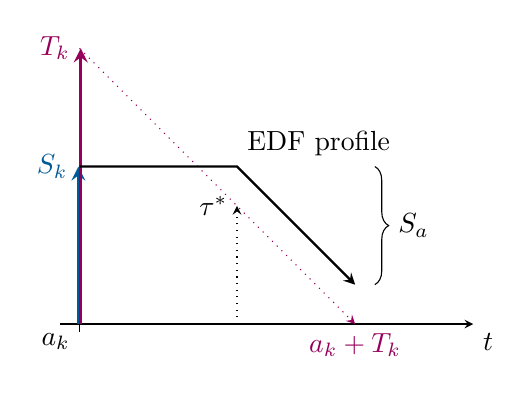
\begin{tikzpicture}[scale=0.5]
	\draw [->] (-.5,0) -- (10,0);
	\node [below right] at (10,0) {$t$};
	\draw [-] (0,-.2) -- (0,.2);
	\node [below left] at (0,0) {$a_k$};
	\draw [very thick,azulcito,->] (-.03,0) -- (-0.03,4) node  [left] {$S_k$};
	\draw [very thick,rojito,->] (.03,0) -- (0.03,7) node  [left] {$T_k$};
	\draw [dotted,rojito,->] (0,7) -- (7,0) node [below] {$a_k+T_k$};
	%\draw [dotted,azulcito,->] (0,4) -- (4,0) node [below] {$a_k+S_k$};
	%immediate scheduling
	\draw [black,thick,->] (0,4) -- (4,4) node[above right] {EDF profile}  -- (7,1);
	\draw [black,dotted,->] (4,0) -- (4,3) node [left] {$\tau^*$};

    \draw [decorate, decoration = {brace,mirror,amplitude=5pt}] (7.5,1) -- node[midway,right, xshift=5pt] {$S_a$} (7.5,4);

\end{tikzpicture}% \tikzsetnextfilename{service_profile_las_lcfs}
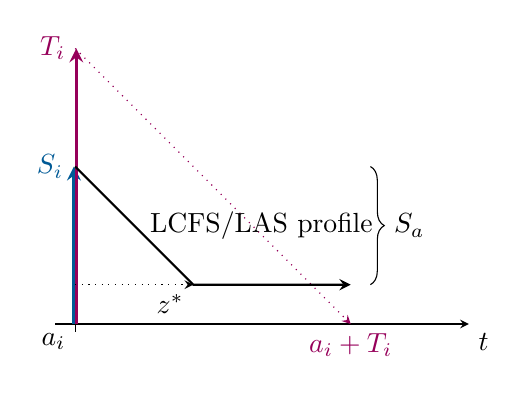
\begin{tikzpicture}[scale=0.5]
	
	\draw [->] (-.5,0) -- (10,0);
	\node [below right] at (10,0) {$t$};
	\draw [-] (0,-.2) -- (0,.2);
	\node [below left] at (0,0) {$a_i$};
	\draw [very thick,azulcito,->] (-.03,0) -- (-0.03,4) node  [left] {$S_i$};
	\draw [very thick,rojito,->] (.03,0) -- (0.03,7) node  [left] {$T_i$};
	\draw [dotted,rojito,->] (0,7) -- (7,0) node [below] {$a_i+T_i$};
	%\draw [dotted,azulcito,->] (0,4) -- (4,0) node [below] {$a_k+S_k$};
	%immediate scheduling
	\draw [black,thick,->] (0,4) -- node [midway, right,xshift=2pt] {LCFS/LAS profile} (3,1) -- (7,1);
	\draw [black,dotted,->] (0,1) -- (3,1) node [below left] {$z^*$};
	\draw [decorate, decoration = {brace,mirror,amplitude=5pt}] (7.5,1) -- node[midway,right, xshift=5pt] {$S_a$} (7.5,4);
\end{tikzpicture}%

	\end{center}

	\bigskip

	Since $\tau^* = x^* = y^* = z^*$, performance is the same in all three policies!!!
\end{frame}

\section{Simulations}



\section{Final remarks}

\begin{frame}{Messages from the talk}
	
\end{frame}

\begin{frame}{Future work}
	
\end{frame}


\begin{frame}[plain]
	\vfill
	{\Huge \alert{Merci beaucoup!}}
	\vfill
	Andres Ferragut

	\smallskip

	\href{mailto://ferragut@ort.edu.uy}{\alert{ferragut@ort.edu.uy}}
	
	\smallskip

	\href{http://aferragu.github.io}{\alert{https://aferragu.github.io}}
\end{frame}

\begin{frame}[allowframebreaks]{References}
	\bibliography{reneging}
\end{frame}
\end{document}
